\documentclass[12pt,letterpaper]{article}

\usepackage{amsmath}               % Enviornments, etc. for typsetting math.
\usepackage{amsthm}                % Theorem/proof enviornments.
\usepackage{amssymb}               % Various symbols.
\usepackage{geometry}              % Easy interface to set page margins.
\usepackage{fancyhdr}              % Custom headers/footers, page styles.
\usepackage[shortlabels]{enumitem} % Stuff for enumerate, itemize environments.
\usepackage{tikz}
\usepackage{stmaryrd}
\usepackage{bbm}
\usepackage{latexsym}
\usepackage{graphicx}
\usepackage{algorithm2e}
\usepackage{mathtools}

\geometry{margin=3cm}              % Sets margins on all sides.
\pagestyle{fancyplain}             % Sets page style.
\headheight 35pt                   % Sets the height of the header.
\headsep 10pt                      % Sets space between the header and the body.

\setlength{\parindent}{0em}        % Sets paragraph indentation.
\setlength{\parskip}{0.5em}        % Sets space between paragraphs.

\setlist[itemize]{leftmargin=*}    % Normalize left margin in itemize. 
\setlist[enumerate]{leftmargin=*}  % Normalize left margin in enumerate.


\newenvironment{solution}{\textit{Solution.}}
\allowdisplaybreaks


\newcommand\semester{Summer 2018}  
\newcommand\banner{AMD}      
\newcommand\E{\mathbb{E}}

\DeclareMathOperator*{\argmax}{arg\,max}

\lhead{\banner}
\chead{\textbf{\Large Midterm Report}}
\rhead{\semester}


\begin{document}

\section{Abstract}
Reinforcement Learning (RL) algorithms are machine learning algorithms which make observations of the environment, take actions and improve their performance from experiences without supervision. Recent studies have shown that RL algorithms can achieve superhuman performance in some areas, such as AlphaGo defeating Lee Sedol in 2016. As powerful as RL algorithms might be, they are sensitive to perturbations in the environment. The goal of this project is to explore the sensitivity of these algorithms and make them more robust. The team first implemented tabular Q-learning with success in simple classic control games. Due to the large state space of images, the team changed the algorithm to deep Q-learning, which produced promising results on a few classic control games and the Atari Breakout game. However, the same architecture failed to yield good performance in a car racing game environment, which demonstrates the fragility of these methods.

% Black-box image
\begin{figure}[h!]
\centering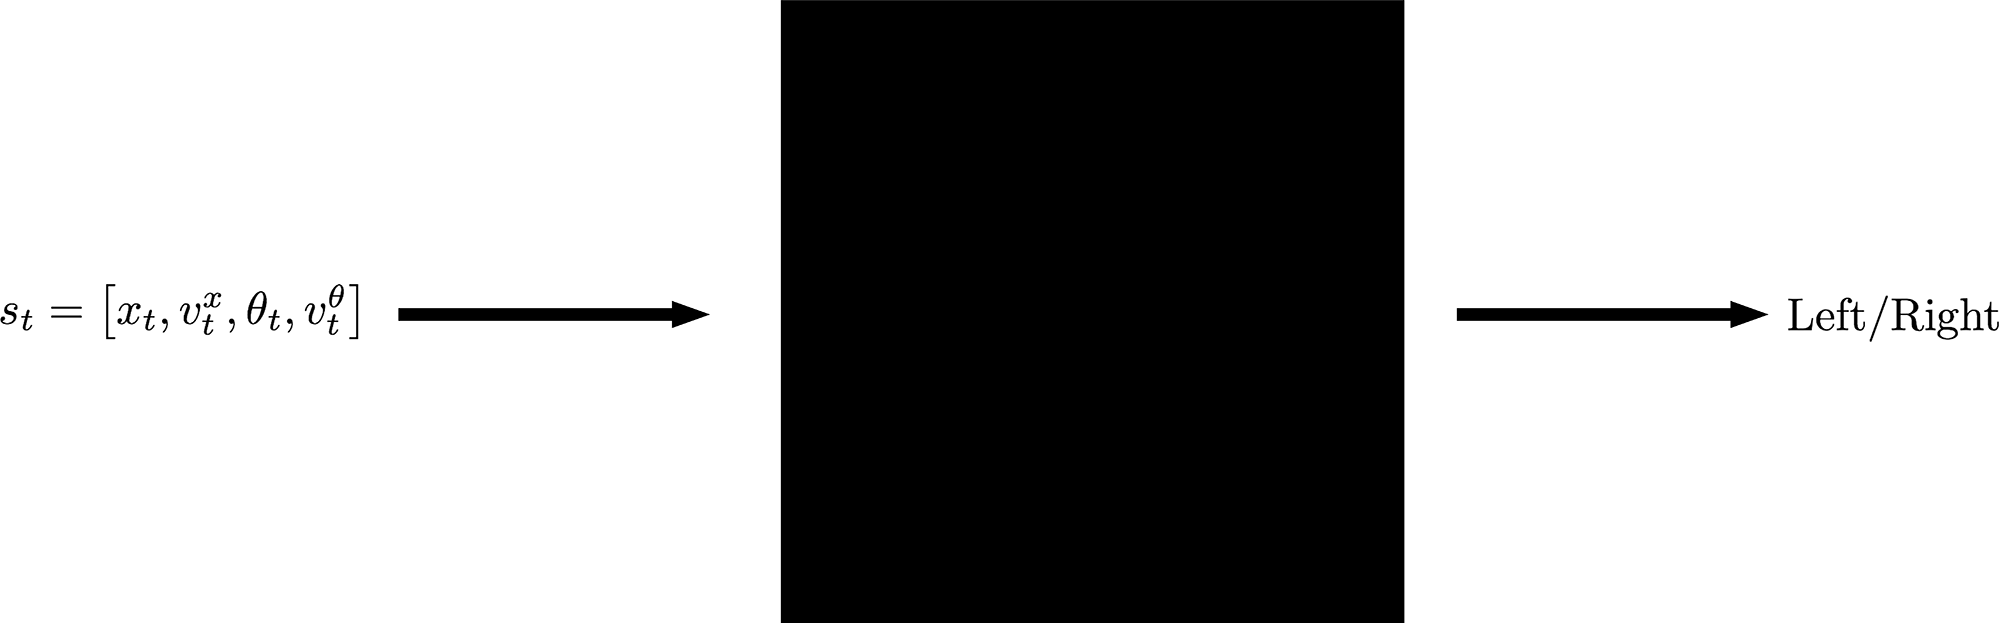
\includegraphics[scale=0.2,clip]{learning_black_box_small.png}
\caption{The black box represents the reinforcement learning algorithm developed: at any given state, the algorithm will output the optimal action.}
\label{fig:black_box}
\end{figure}

% Motivation
\section{Motivation}
Advanced Micro Devices, Inc. (AMD) is an American multinational semiconductor company based in Santa Clara, California, that develops computer processors and related technologies for business and consumer markets. AMD's main products include microprocessors, motherboard chipsets, embedded processors and graphics processors for servers, workstations and personal computers, and embedded systems applications. AMD is interested in developing powerful devices for edge inferencing autonomous vehicles, robotics, manufacturing, and smart grids. Edge inference is the process of infer results of new data from a trained model in an embedded platform. Such platforms are usually limited in computation power. The result of this project could shine light on how the algorithm reacts as new data enters the environment. By exploring the sensitivity of the algorithms, one can gain more intuition about building effective devices for edge inference. \\

Typically, supervised machine learning approaches operate in distinct modes of training and inference. During training, an algorithm is shown labeled data and learns a representation of the underlying distribution of the data. After training, the model can be deployed to provide predictions in a phase known as inference. When such a model is built from layers of computational units called neurons that interact with each other, we call it deep learning. However, supervised machine learning requires labels from human experts, which defeats the purpose of free human from trivial labor. \\

Reinforcement learning is fundamentally different from supervised machine learning. Reinforcement learning is a goal-oriented approach to machine learning and artificial intelligence. The objective of reinforcement learning is to provide a means for an agent to continually learn while dynamically interacting with an environment. As the agent performs actions within the environment, it receives feedback through rewards and learns new behavior.\\

One famous implementation of reinforcement learning is AlphaGo. AlphaGo observed numerous examples of the board game Go in order to learn how a reasonable human would play. It then played against itself and learned to improve its policy through reinforcement learning. As a result, AlphaGo became the first computer program to defeat a Go champion in 2016.\\

Reinforcement learning has also been used in the development of autonomous cars. In 2017, a major automotive company demoed an RC car at the NIPS Conference that dynamically explored and interacted with its environment. As the car explored, it learned more about its environment and how to best navigate it. This is distinct from typical approaches in artificial intelligence which operate in separate modes of training and inference, where an algorithm must first learn by viewing examples of a task being performed before it is capable of making predictions for this same task. \\

Nonetheless, reinforcement learning comes with major flaws. First, reinforcement learning fails in area where it requires long-term strategy. Second, reinforcement learning requires a huge amount of training time and experience. Third, also the main focus of our project, reinforcement learning is not robust to adjust to perturbations in the environment. The goal of this project is to investigate the sensitivity of reinforcement learning algorithms and try to develop a more robust algorithm to adapt to changes in the environment.\\

Reinforcement learning agents learn by exploring their environment 
freely and receiving rewards for ideal behavior. A natural venue
that provides such a sandbox is computer games. Computer games have well-defined environment, action, and reward. These games also do not require a physical device to interact with the environment. We can easily change the environment by varying the parameters of the game settings. Computer games fulfill the criteria for our exploration. We will particularly focus on a car racing game, which is potentially applicable to autonomous cars.


% Basic Q-learning/Tabular Q-learning
\section{Tabular Q-Learning}

\subsection{Q-Learning}
As suggested by figure \ref{fig:black_box}, the aim is to develop a way of
allowing the agent to choose an action at a given state. To accomplish this, a 
function, $Q$, is introduced to map elements from the game's state and action
spaces to the real numbers. In words, $Q(s_t, a_t)$ measures how `good' it is
for the agent to take action $a_t$ when in state $s_t$. 

Given $Q$, an agent can easily determine the best action at state $s_t$ by
computing $Q$ at $s_t$ and every possible action. Thus, with such a $Q$ at hand,
the optimal action is summarized by equation (\ref{eq:optimal_action}).

\begin{align}\label{eq:optimal_action}
\textrm{Action} = \underset{a'}\argmax \; Q(s_t, a_t)
\end{align}

While such a $Q$ is desired, it is not readily available. It will be obtained
by initializing it randomly and allowing the agent to repetitively play the game 
and update $Q$ iteratively. However, at this juncture, the term `good' does not
quantitatively capture whether an action is more favorable than another. To do 
so, the notion of a reward is introduced. 

For every action the agent takes, it will receive a reward, $R_{t+1}$,
indicating whether the  action was immediately favorable -- that is, the reward 
will reflect whether the action was in accordance with the goal of the game. 
Ultimately, rewards serve as a means of informing the agent what it should try
to achieve.

Immediate rewards are constructive for assessing immediate actions, but they fail
to capture the long-term consequences of taking a certain action. Ideally, 
$Q(s_t, a_t)$ represents the expected long-term reward after taking action $a_t$ from
state $s_t$. 

As previously suggested, $Q$ will be obtained iteratively. As such, a method
to update the value of $Q$ at each iteration is needed. To obtain this, the
structure of the sought-after $Q$ must be known. In particular, this $Q$, 
hereafter referred to as $Q^*$, will be defined to capture future rewards. 
Formally, $Q^*$ is as given in equation (\ref{eq:q_star_def})

\begin{align}\label{eq:q_star_def}
Q^*(s_t, a_t) &= \E\left.\left[R_{t+1} + \gamma R_{t+2} +
\gamma^2 R_{t+3} + \cdots = \sum_{i=t}^{\infty} \gamma^{i-t}R_{i+1}
\right|
S = s_t, A = a_t
\right]
\end{align}

where $\gamma \in [0,1]$ is used to determine how much weight is given to future 
rewards. Factoring the right-hand-side of (\ref{eq:q_star_def}) and applying 
the law of total expectation yields equation (\ref{eq:q_star_bellman}),
known as the Bellman equation.

\begin{align}\label{eq:q_star_bellman}
Q^*(s_t, a_t) &= \E\left.\left[R_{t+1} + \gamma \; \underset{a'}\max \; 
Q^*(s_t,a')\right|S = s_t, A = a_t\right]
\end{align}

This splits $Q^*$ into two quantities: the immediate reward and the discounted
future rewards. More importantly,
equation (\ref{eq:q_star_bellman}) reveals an iterative structure that 
immediately yields a suitable iterative update shown in (\ref{eq:q_iter_up}).

\begin{align}\label{eq:q_iter_up}
Q(s_t, a_t)_{j+1} &= Q(s_t, a_t)_j + \alpha \;
\left(R_{t+1} + \gamma \; \underset{a'}\max \; Q(s_t,a') - Q(s_t, a_t)\right)
\end{align}

This update is in the standard iterative update format
$Q(s_t, a_t)_{j+1} = Q(s_t, a_t)_j + \alpha(\textrm{error})$ where
the error captures the difference between what the value $Q(s_t, a_t)$ 
\textit{should} 
be at the current iteration: $R_{t+1} + \gamma \; \underset{a'}\max \; Q(s_t,a')$ 
and what it is at the current iteration: $Q(s_t, a_t)$. It is expected that
as $j \to \infty$, this error term goes to 0. 

Because $Q$ is initialized randomly, immediately taking the actions suggested
by $Q$ as in (\ref{eq:optimal_action}) will introduce bias towards the 
initialization of $Q$. As such, the agent is expected to explore the state space 
and determine which actions are more suitable for certain states. Consequently,
a parameter $\epsilon \in [0,1]$ will be used to determine which action to take
at each iteration: with probability $\epsilon$, a random action will be taken; 
with probability $1 - \epsilon$ the action suggested by $Q$ will be taken.

\subsection{Tabular Representation}
Having established the theoretical aspects of $Q$, it is necessary to find a 
suitable representation that can be found computationally. Two such 
representations will be discussed; here, a tabular representation is
described.

In the tabular setting, $Q$ will be represented by a look-up table where every
row corresponds to a state of the game and the respective columns represent
actions. Due to finite computational memory, storing the value of $Q$ for 
every possible state-action pair is infeasible when state spaces are continuous.
Consequently, continuous parameters from state spaces must be discretized into
disjoint bins. An example of such a discretization is given in figure 
\ref{fig:disc_state_ex} for the game of \textit{CartPole}. 

\begin{figure}[h!]
\centering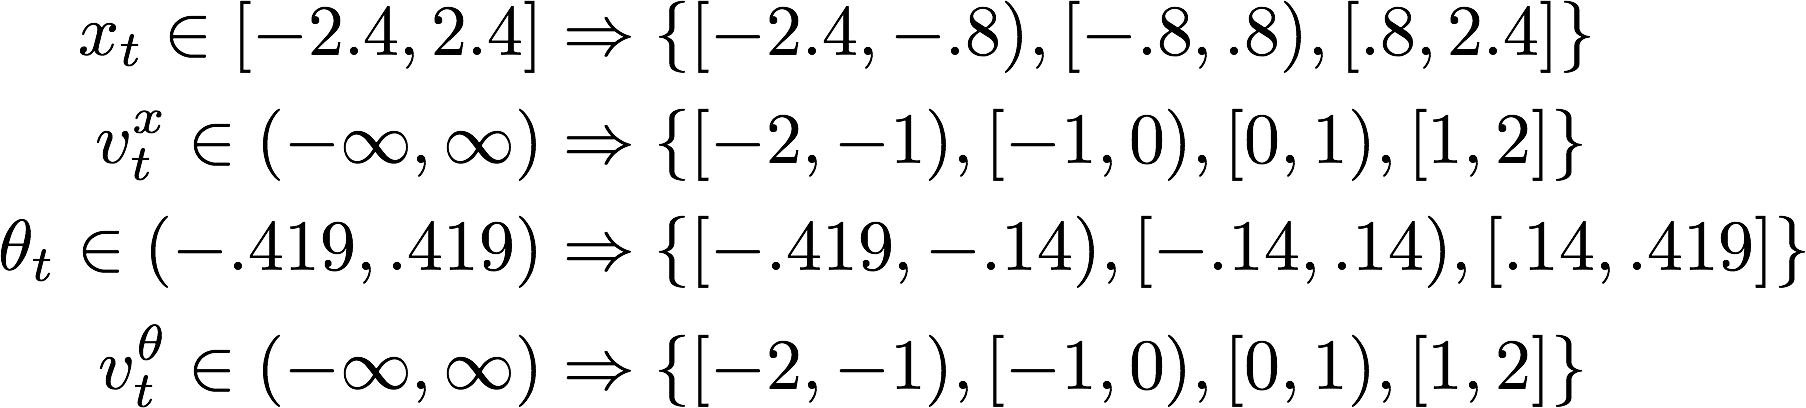
\includegraphics[scale=0.25,clip]{cp_state_disc.png}
\caption{Discretized state space}
\label{fig:disc_state_ex}
\end{figure}

Once the state space has been discretized, each state can be mapped to its
corresponding bin which can then be mapped to a row in the tabular representation
of $Q$. An example of $Q$ for \textit{CartPole} at some iteration is given in 
figure \ref{fig:tab_q_ex}.

\begin{figure}[h!]
\centering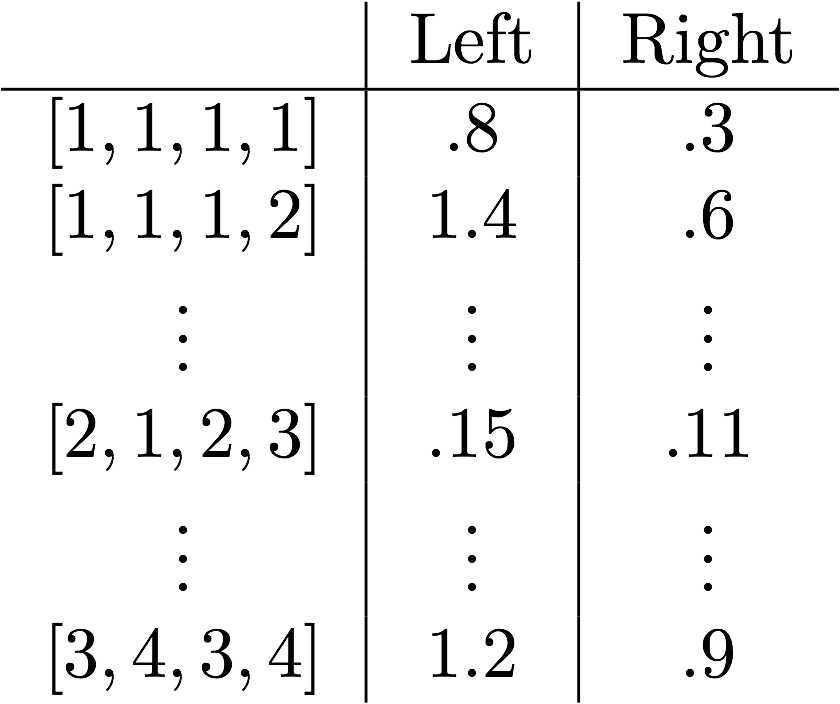
\includegraphics[scale=0.25,clip]{cp_state_lookup_q.png}
 \caption{Tabular $Q$ example}
\label{fig:tab_q_ex}
\end{figure}

\subsection*{Tabular Representation Drawbacks}
While the tabular representation of $Q$ is favorable for pedagogical purposes and 
its implementation ease, it does not generalize well to games with large state 
spaces. For example, a gray-scale image with 1000 pixels has a state space size 
of $256^{1000}$. Storing values for each state is noticeably infeasible. Rather 
than storing the value of $Q$ for every possible state, we will use a function
to approximate $Q$. In particular, we will use a neural network to approximate
$Q$, as discussed in the next section.

% DEEP Q-LEARNING
\section{Deep Q-Learning}
\subsection{Overview}
In this section we outline the Deep Q-Learning (DQN) algorithm, which we took as the starting point 
of our investigation into Deep Reinforcement Learning. The basic idea of DQN is to represent the 
state-action value function Q, as a convolutional neural network. We could of course approximate 
Q by other methods, as there are many function approximation methods out there, but recent work 
has shown deep neural networks to work well in this setting. \\

There are 3 simple modifications one has to make to the tabular Q-Learning algorithm to get what 
now is called the DQN-algorithm, as proposed by the 2013 paper 'Playing Atari with Deep Reinforcement 
Learning' published by DeepMind. We outline these modifications below. 

\subsection{Q as a neural network}
The first step is to replace the function $Q:S\times A \rightarrow \mathbb{R}$ by a neural network \linebreak
${Q(\cdot, \cdot \mid \theta):S \times A \rightarrow \mathbb{R}}$. The resulting network, called 
the Q-network, takes as its input a state and an action, and outputs the estimated Q-value of the 
pair. But the question arises: How do we find good parameters $\theta$ for this model? Suppose that
 at timestep $i$ we have current estimates $\theta_i$ for the weights of the network. The loss
  function we take to be the mean squared TD-error, the same error term as used in the simple 
  tabular Q-learning algorithm, derived from the Bellman optimality equation. 

\begin{align}
L_i(\theta) = \mathbb{E} \left[ \left( R_{t+1} + \gamma\, \max\limits_{a'} Q(s_{t+1}, a' \mid \theta_i) - Q(s_t, a_t \mid \theta) \right)^2 \right]
\end{align}

Since we don't know the dynamics of the environment the agent is operating in, we cannot evaluate 
the above expression, becuase of the expectation operation. We get around this by using Stochastic
Gradient Descent, performing online updates to our estimates of the weights. Using this method,
we get the following update rule for the weights $\theta$ :

\begin{align}
\nabla_{\theta} L_i (\theta) &= \mathbb{E} \left[ \left( R_{t+1} + \gamma\, \max\limits_{a'} Q(s_{t+1}, a' \mid \theta_i) - Q(s_t, a_t \mid \theta) \right) \nabla_{\theta} Q(s_t, a_t \mid \theta ) \right] \\
\theta_{i+1} &= \theta_i - \alpha\, \nabla_{\theta} L_i (\theta) \rvert _{\theta_i}
\end{align}

\subsection{Experience Replay and Fixed Q-Targets}
In theory, Stochastic Gradient Descent only works under some independence assumptions on the data 
we feed it. We need to ask ourselves whether these assumptions are reasonable in this setting. As 
we are playing the game, and updating our weights at each timestep, the sequence of transitions 
visited by the agent is highly correlated: We cannot reasonably expect the game's state to be independent
of its immediate past. Therefore we use the method of experience replay, to decorrelate the data, 
furthermore to achieve higher data efficiency. The method also helps to reduce the risk of getting stuck 
in unwanted feedback loops. \\

At each timestep, we store the tuple $(s_t, a_t, R_{t+1}, s_{t+1})$ in the replay memory denoted by 
$\mathcal{D}$. Instead of updating $\theta$ based on the most recent transition, we instead sample 
uniformly from $\mathcal{D}$, and use these past experiences to perform the gradient descent step with. 
In practice, we sample a minibatch of transitions $(s_j, a_j, R_{j+1}, s_{j+1})_{j \in J}$ where the 
minibatch size $|J|$ is usually chosen to be in the range of 16 to 64. This way we reuse all experiences
 multiple times during training. Another parameter that arises from experience replay is the replay 
 memory capacity - the maximum length of the replay memory - which is chosen in the range of $10^3$ to $10^6$.   

The final modification that needs to be made in order for DQN to work, is the method of fixed Q-targets. 
In the loss function, in the absence of supervision, one must bootstrap from the current weights $\theta_i$ 
in order to arrive at the TD-error, an estimate of Q's accuracy. However, instead of using the most recent 
estimates $\theta_i$, one can use a separate, periodically updated set of weights, usually denoted by $\theta^-$. 
After the modification, the loss function becomes 

\begin{align}
L_i(\theta) = \mathbb{E} \left[ \left( R_{t+1} + \gamma\, \max\limits_{a'} Q(s_{t+1}, a' \mid {\color{red} \theta^-}) - Q(s_t, a_t \mid \theta) \right)^2 \right]
\end{align}


\subsection{DQN summary}
With these methods in place, we are ready to formulate the DQN algorithm: \\
\fbox{
\begin{algorithm}[H]
Initialise $Q$ with random weights $\theta$\\
Set $\theta^- = \theta$. \\
 \For{each episode}{
 Get initial state $s_0$\\
	 \For{t = 1, 2, 3 ... T}{
		Sample $U \sim Unif(0,1)$ \\
		Set $a_t = \begin{dcases}
		    \text{random action sampled uniformly} & \text{if U $< \epsilon$}\\
		    \underset{a'}\argmax \; Q(s_t,a')              & \text{otherwise}
		\end{dcases}$ \\
		Take action $a_t$, get reward $R_{t+1}$ and new state $s_{t+1}$ \\
		Store $(s_t, a_t, R_{t+1}, s_{t+1})$ in the replay memory $\mathcal{D}$\\
		Sample a random minibatch of transitions $(s_j, a_j, R_{j+1}, s_{j+1})$ from $\mathcal{D}$\\
		Set $y_j = \begin{dcases}
		    R_{j+1} + \gamma\, \max\limits_{a'} Q(s_{j+1}, a';\theta^-)& \text{if $s_{j+1}$ is not terminal} \\
		    R_{j+1},              & \text{otherwise}
		\end{dcases}$ \\
		Perform a gradient descent step on the loss $\left( y_j - Q(s_j, a_j;\theta)\right)^2$ \\
		Every C steps set $\theta^- = \theta$. 
 	}
 }
\end{algorithm}
}

\begin{figure}[h!]
\centering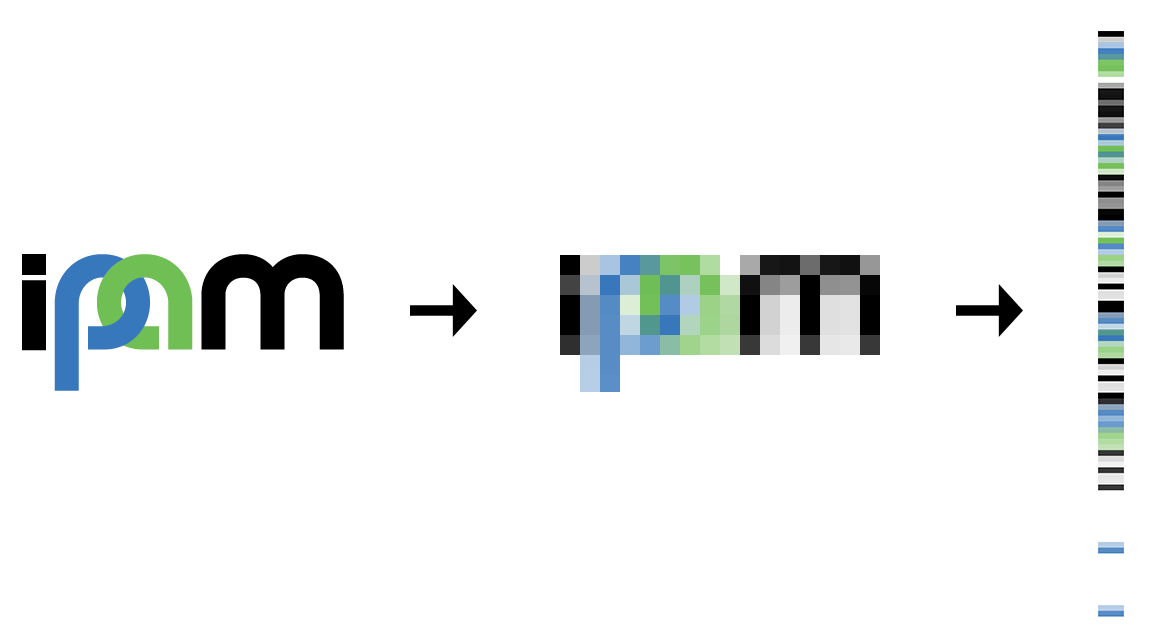
\includegraphics[scale=0.25,clip]{ipam.png}
\caption{Downsampling and flattening the logo of IPAM}
\label{fig:ipam}
\end{figure}

\subsection{DQN in practice}
So far we haven't talked about how the agent internally represents the game's state. 
In the more complex computer games we consider, the only observation the agent is given 
by its environment is an RGB image of the screen for each frame of the game. We process these images, 
in order to be able to use them as input to the Q-network. We do so following the methods of
the DeepMind paper 'Playing Atari with Deep Reinforcement Learning'. 
At each timestep, take the most recent 4 frames, convert them to grayscale, downsample to a size 
of about 80x80, and then stack them to produce the input to the network. See figure \ref{fig:ipam} 
for a partial visualisation of the process. 


\section{Results}
\subsection{Tabular Q-Learning for Classic Control Games}

\begin{figure}[h!]
\centering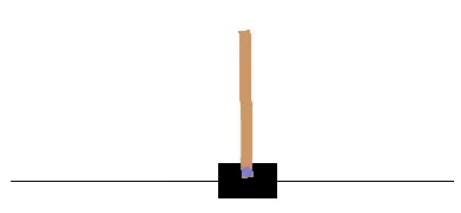
\includegraphics[scale=0.45,clip]{cartpole.png}
\caption{Cart Pole}
\label{fig:cartpole}
\end{figure}

The  team initially investigated two simple games from the OpenAI Gym toolkit. The first game was Cart Pole, where the goal is to balance a pole in a cart for as long as possible. In this game, the state is represented as a four-dimensional vector containing the values for the position of the cart, the velocity of the cart, the angle of the pole, and the velocity of the pole. The game is considered solved when the agent achieves an average score $\geq$ 195 over 100 consecutive trials. Using the tabular Q-learning approach, the algorithm achieved a perfect score of 200 over 100 consecutive trials. This score was achieved with a bucket size of 1 for the position and velocity of the cart and a bucket size of 20 for the angle and velocity of the pole for state space discretization. This agent was trained for 500 episodes with a discount factor of 0.99, minimum learning rate of 0.05, and minimum explore rate of 0.1.

\begin{figure}[h!]
\centering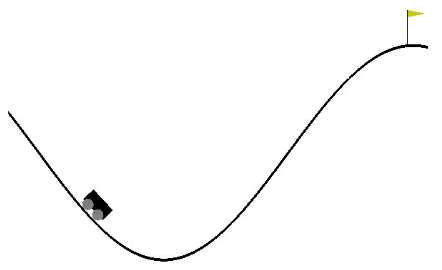
\includegraphics[scale=0.45,clip]{mountain_car.png}
\caption{Mountain car}
\label{fig:mountain_car}
\end{figure}

The team also trained the tabular Q-learning algorithm for the Mountain Car game. In this game, the goal is for the car to reach the top of the mountain as quickly as possible. The team initially faced challenges with this game due to the nature of the reward function. Since the reward function returns a negative reward for each time step, it is difficult to reinforce positive behavior before actually winning the game. As a result, the performance varied as a result of slight changes in parameters. After experimentation, the algorithm performed best with a bucket size of 10 for position, bucket size 30 for velocity, discount factor of 0.99, fixed learning rate of 0.05 and fixed explore rate of 0.1. After training for 10,000 episodes, the algorithm achieved an average reward of -157.64 over 100 test episodes.

\subsection{Deep Q-Learning for Breakout}
The team then implemented the Deep Q-Learning algorithm on the Atari Breakout game using a neural network. The first layer of the neural network was a convolutional layer with 32 kernels, 8x8 filter, and stride 4x4. The second was a convolutional layer with 16 kernels, 4x4 filter, and stride 2x2. The third layer was a dense layer with 256 neurons and a nonlinear rectifier. The final layer was a dense layer with 16 neurons and a linear rectifier. The performance was quantitatively analyzed using average Q-values. Assuming that $S$ is a uniform sample of $n$ fixed states, an estimate of the average Q-value was computed as follows.
$$ Q_{avg} = \frac{1}{n} \sum_{i=1}^{n} max_{a} Q(s_{i},a) ~~~ s_{i} \in S$$

Using this architecture, the algorithm was able to achieve promising results on Breakout as shown in \ref{fig:breakout}. The average Q-value appeared to increase over time and eventually converge.

\begin{figure}[h!]
\centering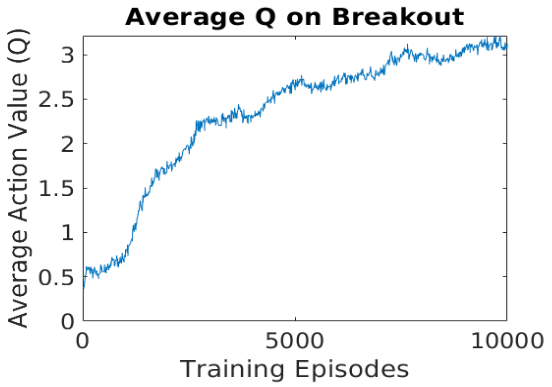
\includegraphics[scale=0.5,clip]{breakout_q.png}
\caption{Average Q Plot for Breakout}
\label{fig:breakout}
\end{figure}



\subsection{Deep Q-Learning for Car Racing}

\begin{figure}[h!]
\centering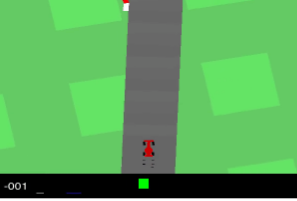
\includegraphics[scale=0.5,clip]{car_racing.png}
\caption{Car Racing}
\label{fig:car_racing}
\end{figure}

The team attempted to train the Deep Q-Learning algorithm on the Car Racing game using the same neural network architecture used for Breakout. However, the algorithm was unable to achieve good performance in the Car Racing game with this approach. This failure demonstrates the fragility of these reinforcement learning methods and provides motivation for the goals of this project.

In order to gain a better understanding of why the algorithm fails in this environment, the team simplified the Car Racing game to a fixed straight racetrack. The algorithm was successful in learning the simple task of moving forward at all times. This indicates that the algorithm has the potential to learn in the Car Racing environment. It is possible that a change in architecture or approach could lead to better performance.

\section{Next Steps}
The team would like to improve the performance of the Deep Q-Learning algorithm on the Car Racing game. One approach is to adjust the reward function by putting more emphasis on positive reward rather than negative reward. Another approach is to utilize curriculum training by teaching the algorithm simple tasks and slowly introducing more difficult tasks. Once the algorithm can successfully compete in the Car Racing environment, perturbations will be introduced into the environment to analyze performance of the agent in configurations of the environment that it has not seen in training. If time permits, the team aims to make adjustments to the Deep Q-Learning algorithm to make it more robust. Such adjustments could include batch normalization or regularization, which could prevent over-fitting in the learning model. Further experimentation with neural network architectures may also be considered.





\end{document}